$\displaystyle \int_{6}^{9}\frac{3\ln x-5}{x}\,dx$

\nopagebreak
\begin{align*}
I &= \int_{6}^{9} \left( 3 \frac{\ln x}{x} - \frac{5}{x} \right) dx \\
&= 3 \int_{6}^{9} \frac{\ln x}{x} dx - 5 \int_{6}^{9} \frac{dx}{x} \\
\text{Para la primera integral: } & u=\ln x, du=dx/x. \\
I &= 3 \left[ \frac{(\ln x)^2}{2} \right]_{6}^{9} - 5 \left[ \ln|x| \right]_{6}^{9} \\
&= \frac{3}{2} ((\ln 9)^2 - (\ln 6)^2) \\
&\quad - 5 (\ln 9 - \ln 6) \\
&= \frac{3}{2} ((\ln 9)^2 - (\ln 6)^2) - 5 \ln \frac{3}{2}
\end{align*}

\[
\boxed{\displaystyle \frac{3}{2} ((\ln 9)^2 - (\ln 6)^2) - 5 \ln \frac{3}{2}}
\]

\begin{center}
    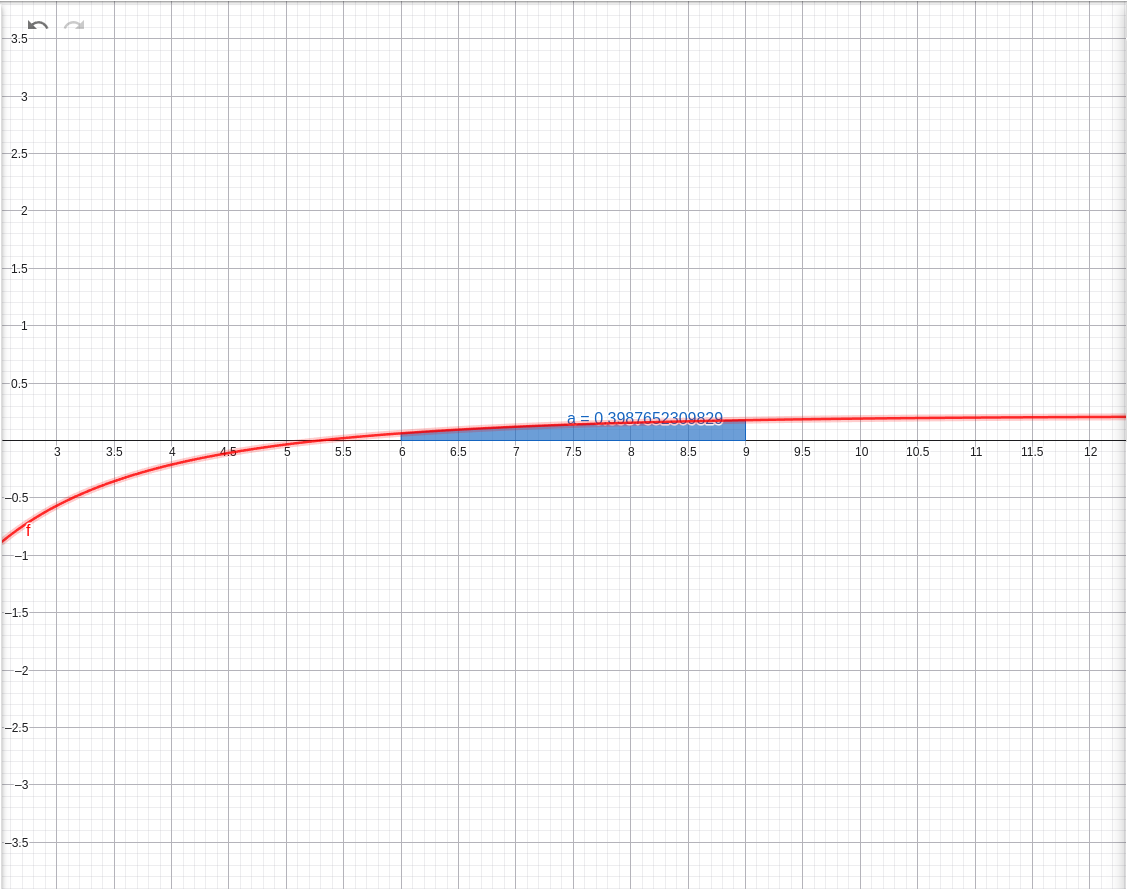
\includegraphics[width=0.5\textwidth]{Graficas/ejer15.png}
\end{center}
